\section{The microtubule}
I am going to add more description of the microtubule here. \\

Dynein walks along a particular cyctoskeleton filament called a microtubule which has an inherent structural polarity identified as the plus ($+$) and minus ($-$) ends \cite{lodish_microtubule_2000}. Most(not all) variations of the kinesin molecular motor are plus-end directed whereas dynein is only minus-end directed \cite{alberts_molecular_2002}. \\

I intend to discuss how our model may elucidate why dynein is specifically directed towards the minus end. 

\section{The powerstroke model} 
Here I will talk about the powerstroke vs winch mechanism debate. 

\section{Observations \textit{in vitro}} 
Here I will talk about how single-molecule observations are made as well as their limitations (e.g. can't observe stutter steps of $0$ $nm$.) \\\\

Naturally, one might wonder at how such small motors can be studied in the laboratory. Kinesin and Dynein have masses of a few hundred kDa and  $\sim2$ MDa respectively \cite{liao_kinesin_1998, johnson_structure_1983}. Recalling that 1 Dalton (Da) corresponds to one atomic mass unit means these proteins consist of, at most, a few million atoms. This small scale poses a unique experimental challenge. One way this is approached at OSU by Prof. Weihong Qiu's group is by attaching small fluorescent molecules called fluorophores to the binding sites that motor proteins use to latch onto their cargo. Then, the individual movement of motors is tracked using total internal reflection fluorescence microscopy to produce video of the proteins in action as illustrated in figure \ref{fig:weihong tirf} from \cite{qiu_dynein_2012}. 

\begin{figure}[!hbt]
	\centering
	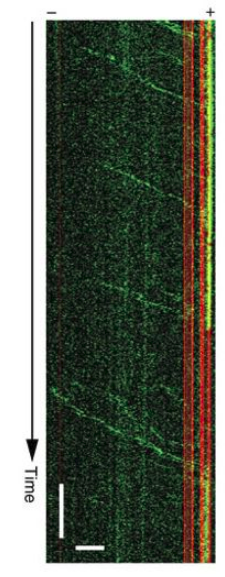
\includegraphics[angle=90, width=0.75\columnwidth]{weihong_motor}
	\caption{\textbf{TIRF Microscopy Imaging} individual kinesin proteins are imaged as small green dots and tracked as they move. Slices at different times are stacked so that the slope of each green line indicates the velocity of the protein. Image taken from \cite{qiu_dynein_2012}.}
	\label{fig:weihong tirf}
\end{figure}

Although the individual binding domains of the molecule can not be resolved, 
\section{Transporting cargo}
\section{Experimental stepping statistics}
Here I will include the various stepping statistics (distribution, binding/unbinding rates, etc...) that we hope to  


\section{More motivation} 
Here I will discuss other simulation efforts that, in our opinion, make far to many assumptions or are purely monte carlo and don't actually simulate the motion of the protein. I will also discuss why our simulation is a happy medium between a full on molecular dynamics simulation (time expensive but accurate) and monte carlo (very fast but doesn't dynamically simulate the protein and instead just selects steps from a distribution). 